\documentclass[12pt]{ociamthesis}  % default square logo 
%\documentclass[12pt,beltcrest]{ociamthesis} % use old belt crest logo
%\documentclass[12pt,shieldcrest]{ociamthesis} % use older shield crest logo

%load any additional packages
\usepackage{amssymb}
\usepackage{listings}

\usepackage{color}
 
\definecolor{codegreen}{rgb}{0,0.6,0}
\definecolor{codegray}{rgb}{0.5,0.5,0.5}
\definecolor{codepurple}{rgb}{0.58,0,0.82}
\definecolor{backcolour}{rgb}{0.95,0.95,0.92}
 
\lstdefinestyle{mystyle}{
    backgroundcolor=\color{backcolour},   
    commentstyle=\color{codegreen},
    keywordstyle=\color{magenta},
    numberstyle=\tiny\color{codegray},
    stringstyle=\color{codepurple},
    basicstyle=\footnotesize,
    breakatwhitespace=false,         
    breaklines=true,                 
    captionpos=b,                    
    keepspaces=true,                 
    numbers=left,                    
    numbersep=5pt,                  
    showspaces=false,                
    showstringspaces=false,
    showtabs=false,                  
    tabsize=2,
    language=python
}
 
\lstset{style=mystyle}
%input macros (i.e. write your own macros file called mymacros.tex 
%and uncomment the next line)
%\include{mymacros}

\title{Tugas \\[1ex]     %your thesis title,
        Kecerdasan Buatan 1}   %note \\[1ex] is a line break in the title

\author{Dzul Jalali Wal Ikram}             %your name
\college{1194011}  %your college

%\renewcommand{\submittedtext}{change the default text here if needed}
\degree{Politeknik Pos Indonesia}     %the degree
\degreedate{Bandung 2022}         %the degree date

%end the preamble and start the document
\begin{document}

%this baselineskip gives sufficient line spacing for an examiner to easily
%markup the thesis with comments
\baselineskip=18pt plus1pt

%set the number of sectioning levels that get number and appear in the contents
\setcounter{secnumdepth}{3}
\setcounter{tocdepth}{3}


\maketitle                  % create a title page from the preamble info
\include{section/dedication}        % include a dedication.tex file
\include{section/acknowlegements}   % include an acknowledgements.tex file
\include{section/abstract}          % include the abstract

\begin{romanpages}          % start roman page numbering
\tableofcontents            % generate and include a table of contents
\listoffigures              % generate and include a list of figures
\end{romanpages}            % end roman page numbering

%now include the files of latex for each of the chapters etc
\chapter{Mengenal Kecerdasan Buatan dan Scikit-Learn}

\section{Teori}
Praktek teori penunjang yang dikerjakan :
\begin{enumerate}
	\item Sejarah Perkembangan dan penjelasan Definisi \textit{Artifical Intelligence}. \textit{Artifical Intelligence} merupakan suatu ilmu pada bidang komputer yang memiliki 
	kemampuan untuk meniru, melakukan sesuatu sama seperti yang dilakukan oleh manusia.\\
	Pada akhir tahun 1955 program \textit{Artifical Intelligence} pertama kali muncul berkat adanya perkembangan \textit{The Logic Theorist} oleh Newell dan Simon. 
	Program tersebut menunjukan masalah dengan menggunakan model pohon, dimana untuk menyelesaikannya hanya perlu memilih sebuah cabang yang akan menghasilkan sebuah kesimpulan yang paling
	benar. Dengan adanya program tersebut pengembangan dibidang  \textit{Artifical Intelligence} mengalami peningkatan yang besar. Di tahun 1956, seseorang bernama John McCarthy dari 
	Massacuhetts Institute of Technology yang juga dikenal sebagai Bapak AI, menyelenggarakan sebuah konferensi dengan nama \textit{The Dartmouth summer research project on artificial intelligence},
	konferensi itu diselenggarakan untuk menarik minat para ahli komputer untuk berkumpul dan bertemu. Konferensi tersebut mempertemukan para pendiri dibidang AI dan bertugas untuk meletakan
	dasar untuk penelitian dan pengembangan \textit{Artifical Intelligence} dimasa depan.
	
	\item Definisi supervised learning, klasifikasi, regresi dan unsupervised learning. Data set, training set dan testing set
	\begin{itemize}
		\item Supervised Learning
		\par
		\textit{Supervised learning}
		adalah suatu pendekatan machine learning yang ditentukan berdasarkan penggunaan dataset, supervised learning menggunakan dataset berlabel atau labeled dataset. Supervised Learning digunakan untuk melakukan klasifikasi data atau memprediksi hasil secara akurat sesuai dengan output berdasarkan pola yang ada didalam data training dan berupa data yang memiliki label yang sudah ditentukan terlebih dahulu
		\item Unsupervised Learning
		\par
		\textit{Unsupervised Learning} adalah pendekatan machine learning yang digunakan untuk menganalisa dan juga mengelompokan kumpulan - kumpulan data yang tidak berlabel.
		\item Klasifikasi
		\par
		\textit{Klasifikasi} adalah sebuah proses menggunakan algoritma untuk secara akurat memasukan data kedalam kategori yang spesifik.
		\item Regresi
		\par
		\textit{Regresi} adalah sebuah proses menggunakan algoritma untuk memahami hubungan antara 2 variabel, yaitu variabel dependen dan variabel independen, Regresi dapat memprediksi nilai numerik variabel dependen berdasarkan variabel independen.
		\item Dataset
		\par
		\textit{Dataset} adalah suatu kumpulan data yang berisi informasi-informasi lama, dan dapat dikelola sehingga menjadi sebuah informasi baru.
		\item Training set
		\par
		\textit{Training set} adalah bagian dari dataset yang dilatih untuk kemudian digunakan untuk memprediksi sesuatu atau menjalankan fungsi dari algoritma.
		\item Testing set
		\par
		\textit{Testing set} adalah bagian dari dataset yang digunakan untuk melihat tingkat keakuratan dan performa dari algoritma.
	\end{itemize}

\end{enumerate}


\section{Instalasi}

\begin{enumerate}
\item Melakukan installasi pada anaconda promt dengan perintah " pip install -U scikit-learn".
\begin{figure}[!htbp]
	\centering
	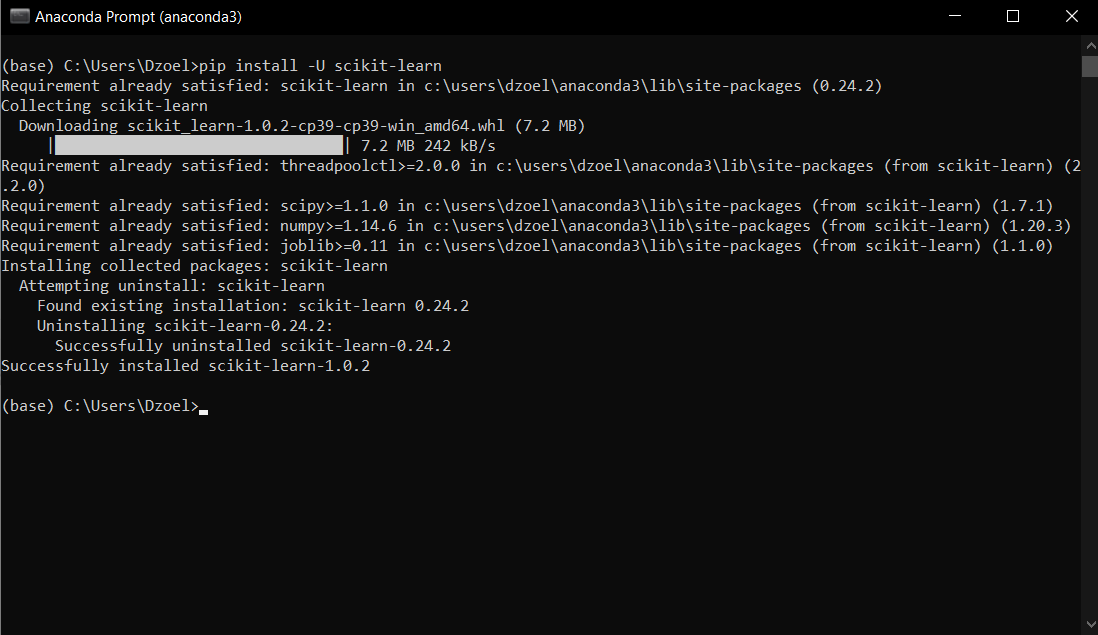
\includegraphics[scale=0.4]{figures/pipinstall.PNG}
\end{figure}
\newpage
\item Kemudian klik link berikut ini untuk melakukan basic tutorial \textit{scikit-learn} "https://scikit-learn.org/stable/tutorial/basic/tutorial.html".
\item
Mencoba Loading an example dataset
\begin{figure}[!htbp]
	\centering
	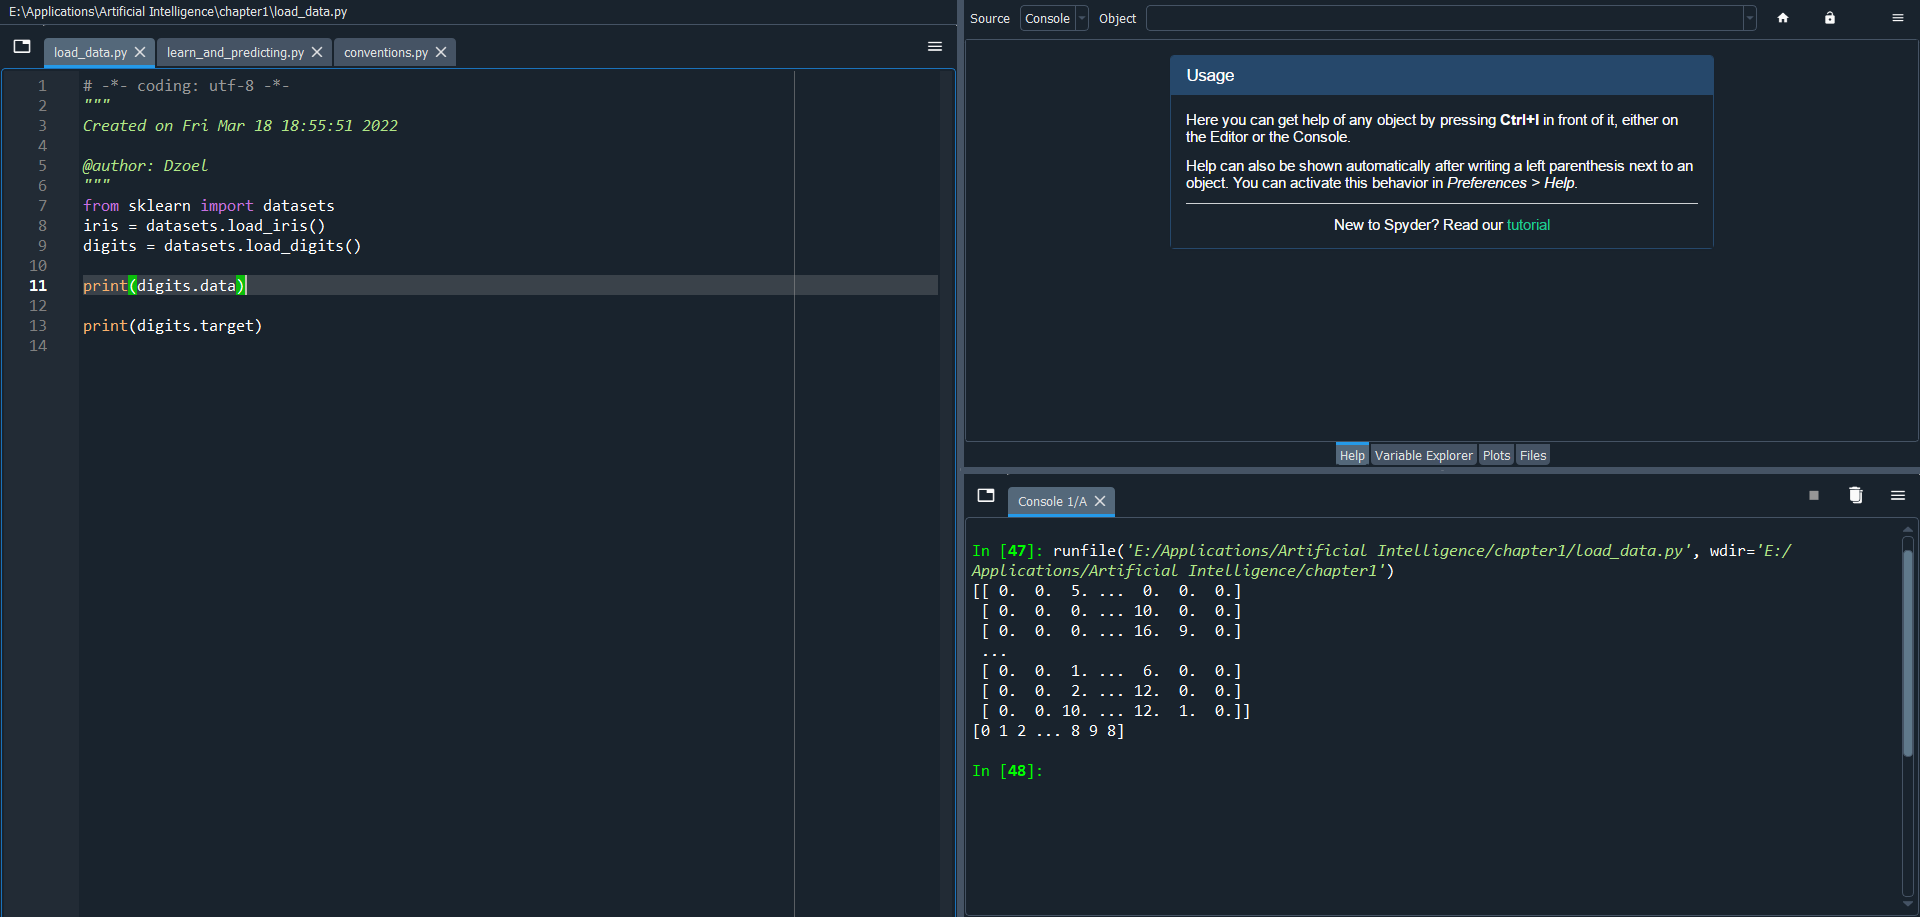
\includegraphics[scale=0.4]{figures/loaddataset.PNG}
\end{figure}
\item
Mencoba Learning and predicting
\begin{figure}[!htbp]
	\centering
	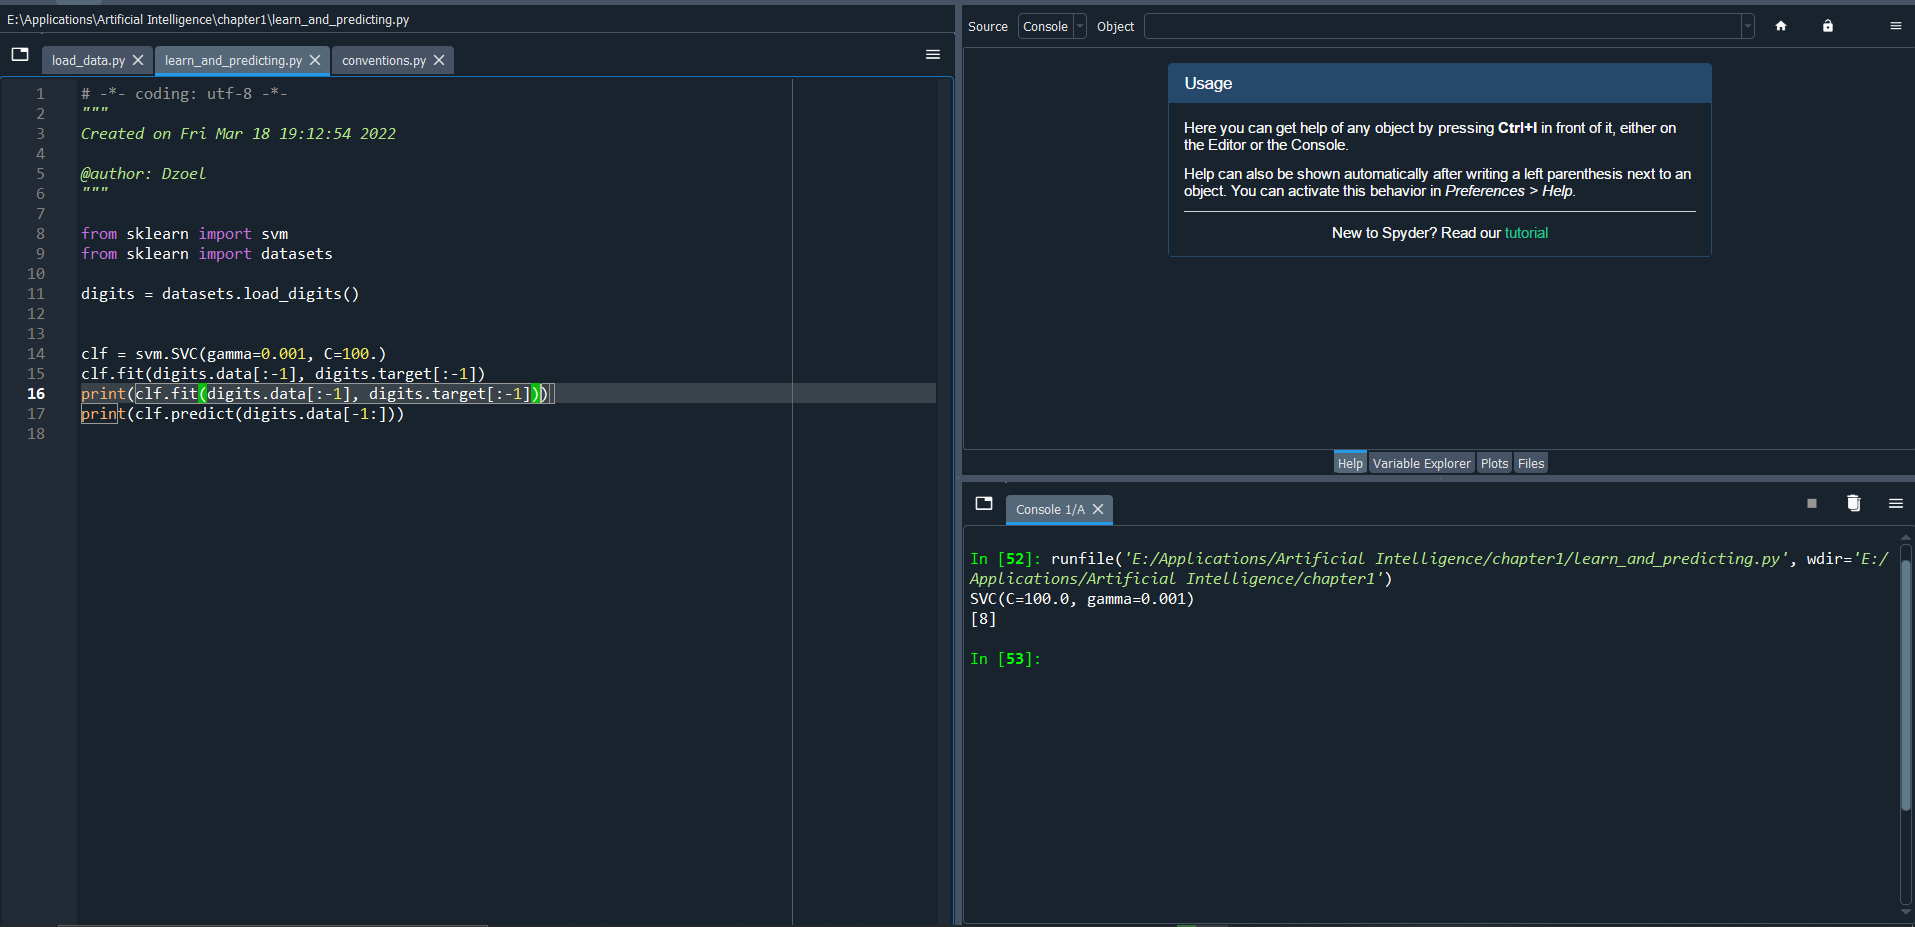
\includegraphics[scale=0.4]{figures/learnpredict.PNG}
\end{figure}
\newpage
\item 
Mencoba Conventions
\begin{figure}[!htbp]
	\centering
	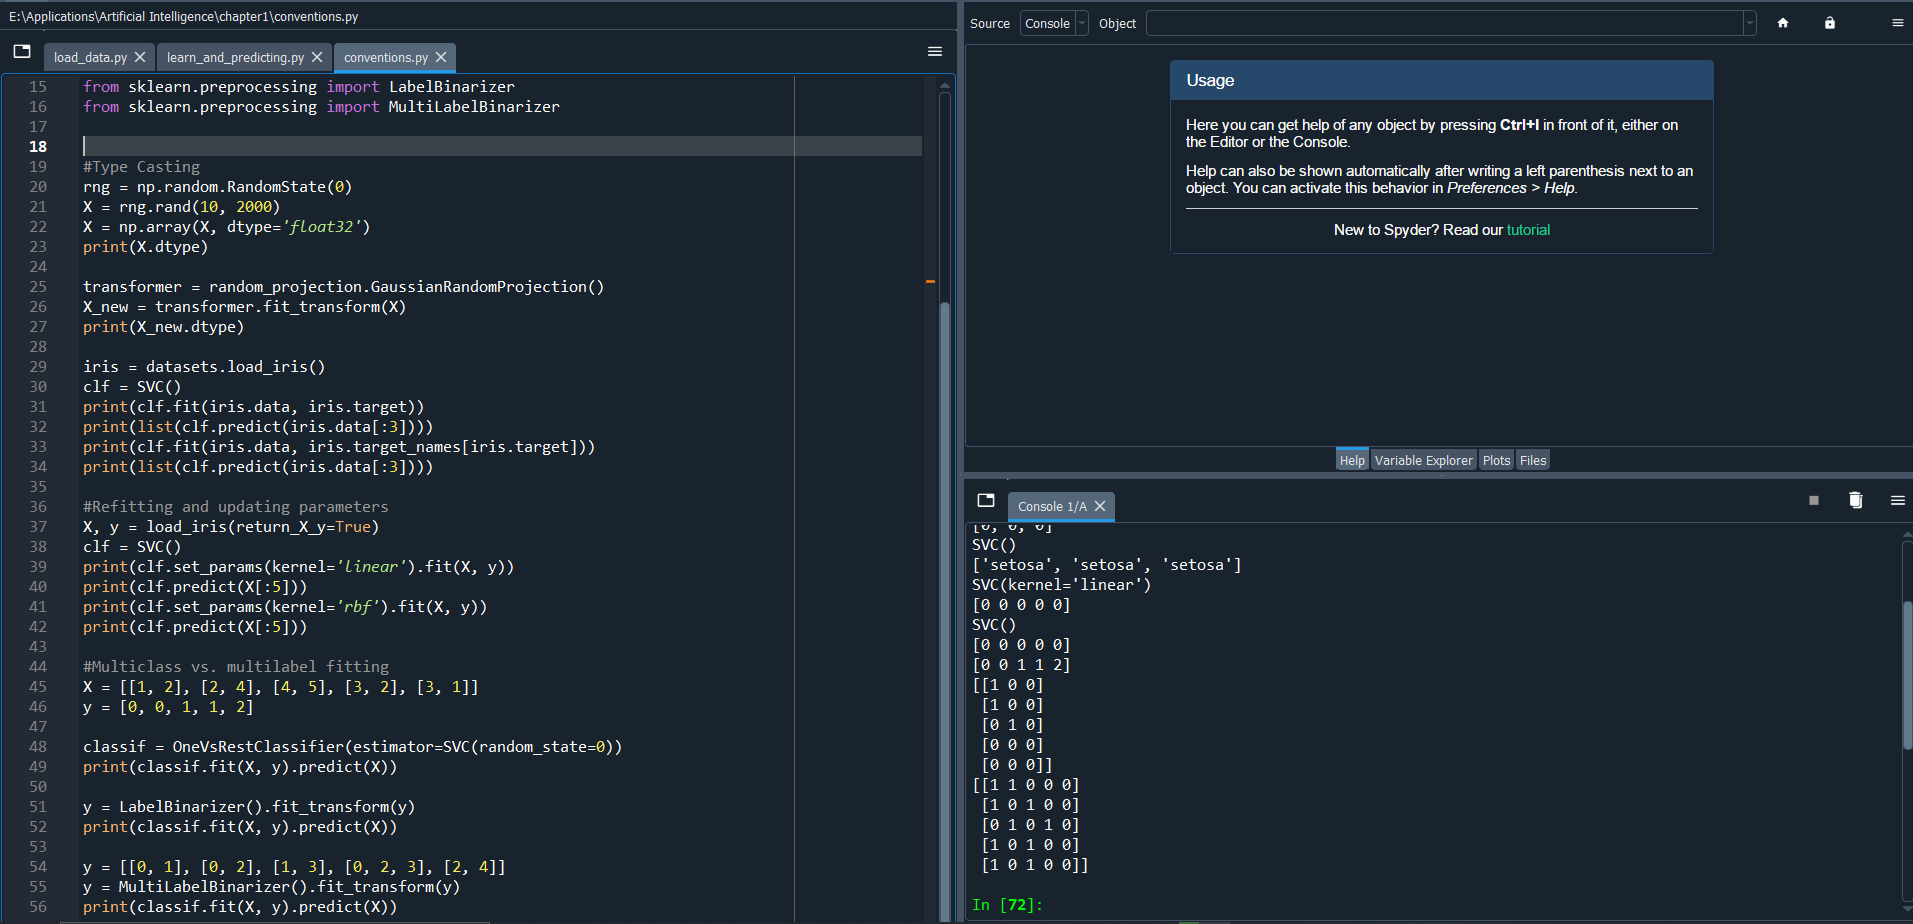
\includegraphics[scale=0.4]{figures/convention.PNG}
\end{figure}
\newpage
\item Link Youtube praktikum : https://www.youtube.com/watch?v=tFsRdpQ-VUg
\end{enumerate}


\section{Penanganan Error}
Dari percobaan yang dilakukan di atas, apabila mendapatkan error maka:

\begin{enumerate}
\item Screenshoot Error
\begin{figure}[!htbp]
	\centering
	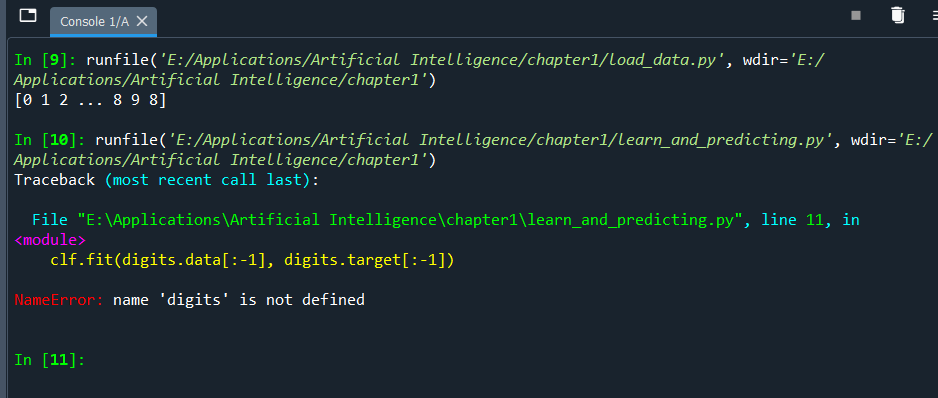
\includegraphics[scale=0.6]{figures/nameError.PNG}
\end{figure}
\begin{figure}[!htbp]
	\centering
	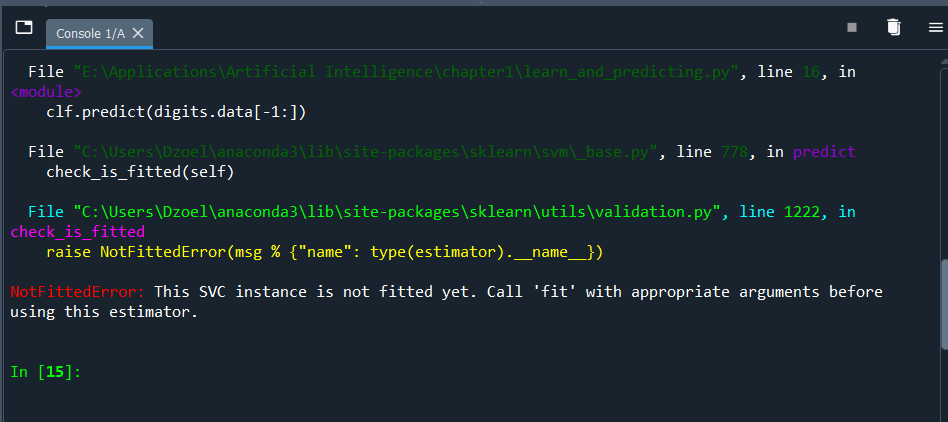
\includegraphics[scale=0.6]{figures/notfittederror.PNG}
\end{figure}

\newpage    
\item Tuliskan kode error dan jenis error
\par 
NameError = name 'digits' is not defined
\par
NotFittedError = This SVC instance is not fitted yet. Call 'fit' with appropriate arguments before using this estimator.

	\item
Solusi pemecahan masalah error tersebut
\par
NameError = solusinya adalah membuat variabel dengan nama digits
\par
NotFittedError = solusinya adalah memanggil parameter dengan method fit, sebelum menggunakan method predict.

\end{enumerate}


\chapter{Membangun Model Prediksi}

\section{Teori}
Praktek teori penunjang yang dikerjakan(nilai 5 per nomor, untuk hari pertama) :
\begin{enumerate}
\item
Jelaskan apa itu binary classification dilengkapi ilustrasi gambar sendiri \\
\textit{Binary Classification} adalah mengklasifikasikan elemen - elemen himpunan menjadi 2 kelompok berdasarkan aturan klasifikasi.
\item
Jelaskan apa itu supervised learning dan unsupervised learning dan clustering dengan ilustrasi gambar sendiri. \\
\begin{itemize}
	\item Supervised Learning
	\par
		\textit{Supervised Learning} adalah suatu pendekatan machine learning yang ditentukan berdasarkan penggunaan dataset, supervised learning menggunakan dataset berlabel atau labeled dataset. Supervised Learning digunakan untuk melakukan klasifikasi data atau memprediksi hasil secara akurat sesuai dengan output berdasarkan pola yang ada didalam data training dan berupa data yang memiliki label yang sudah ditentukan terlebih dahulu. \\
		\begin{figure}[!htbp]
			\centering
			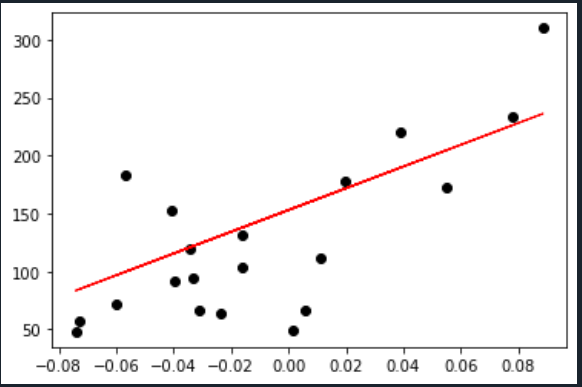
\includegraphics[scale=0.4]{figures/supervised-learning.PNG}
		\end{figure}
		\newpage
	\item Unsupervised Learning
	\par
		\textit{Unsupervised Learning} adalah pendekatan machine learning yang digunakan untuk menganalisa dan juga mengelompokan kumpulan - kumpulan data yang tidak berlabel.\\
		\begin{figure}[!htbp]
			\centering
			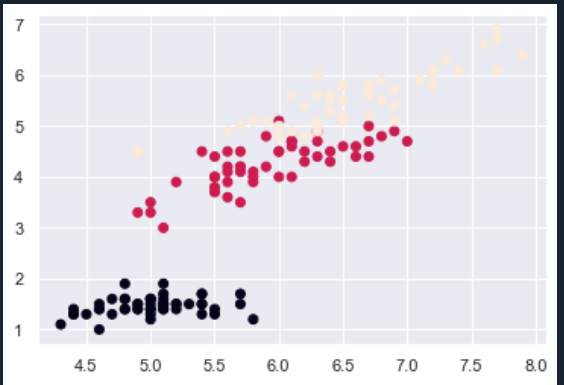
\includegraphics[scale=0.4]{figures/unsupervised-learning.PNG}
		\end{figure}
	\item Clustering
	\par
	\textit{Clustering} adalah sebuah proses pengelompokan data kedalam beberapa cluster sehingga data-data disuatu cluster memiliki kemiripan.\\
	\begin{figure}[!htbp]
		\centering
		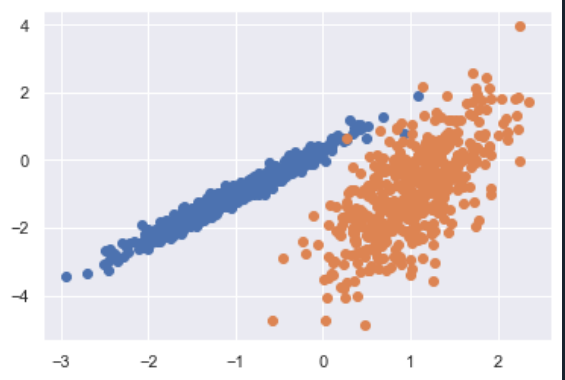
\includegraphics[scale=0.4]{figures/clustering.PNG}
	\end{figure}
	\par
	\item
	Jelaskan apa itu evaluasi dan akurasi dari buku dan disertai ilustrasi contoh dengan gambar sendiri
	\par
	\item 
	\textit{Evaluasi dan Akurasi}
	Evaluasi adalah bagaimana cara agar dapat mengevaluasi seberapa baiknya model bekerja dengan cara mengukur akurasinya.\\
	Akurasi memiliki definisi sebagai persentase kasus yang diklasifikasikan dengan benar.\\
	Kesalahan dari model dapat dianalisi menggunakan confusion matrix.\\
	\par
	\item
	Jelaskan bagaimana cara membuat dan membaca confusion matrix, buat confusion matrix buatan sendiri.
	\par
	\item 
	\textit{Confusion Matrix}\\ 
	1. Import dependencies yang dibutuhkan.\\
	2. Kemudian buat variabel untuk menampung value atau Nilai yang diprediksi.\\
	3. Buat variabel untuk menampung value atau nilai sebenarnya.\\
	4. Kemudian print confusion matrixnya dengan menggunakan variabel dari nilai sebenarnya dan variabel nilai yang diprediksi dengan label misalnya a,b,c.\\
	5. Kemudian print precision dan recall diantara matrix lainnya.
	\begin{figure}[!htbp]
		\centering
		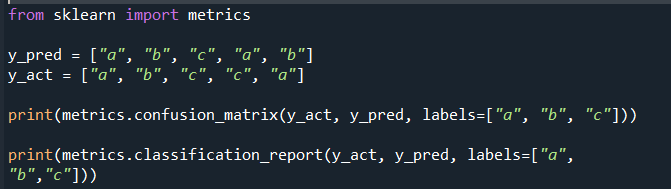
\includegraphics[scale=0.8]{figures/confusionmatrix.PNG}
	\end{figure}
	\begin{figure}[!htbp]
		\centering
		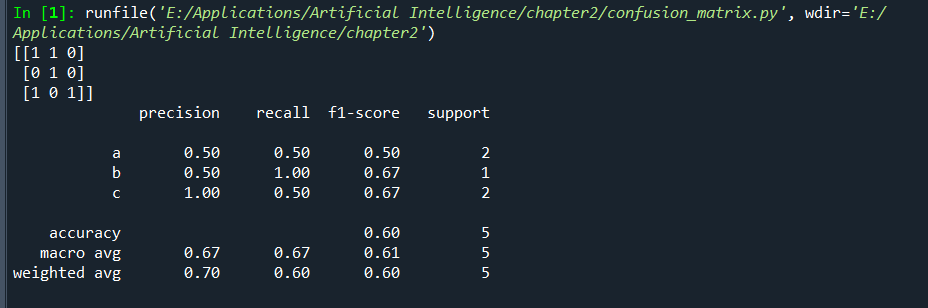
\includegraphics[scale=0.6]{figures/hasilconfusionmatrix.PNG}
	\end{figure}
	\item
	Jelaskan bagaimana K-fold cross validation bekerja dengan gambar ilustrasi contoh buatan sendiri.\\
	\item 
	1. Mengacak dataset secara random.\\
	2. Membagi dataset tersebut kedalam k-group, yaitu sebagai test dataset dan sisanya sebagai training dataset.\\
	3. Pasang model di set pelatihan dan evaluasi di set tes.\\
	4. Simpan skor evaluasi dan buang modelnya.\\
	5. Meringkas keterampilan model menggunakan sampel skor menggunakan model evaluasi.
	\item
	Jelaskan apa itu decision tree dengan gambar ilustrasi contoh buatan sendiri.
	\item 
	\textit{Decision Tree} adalah metode yang digunakan untuk membantu membuat keputusan dengan menggunakan model pohon untuk menampilkan keputusan, kemungkinan resiko, dan lainnya.
	\begin{figure}[!htbp]
		\centering
		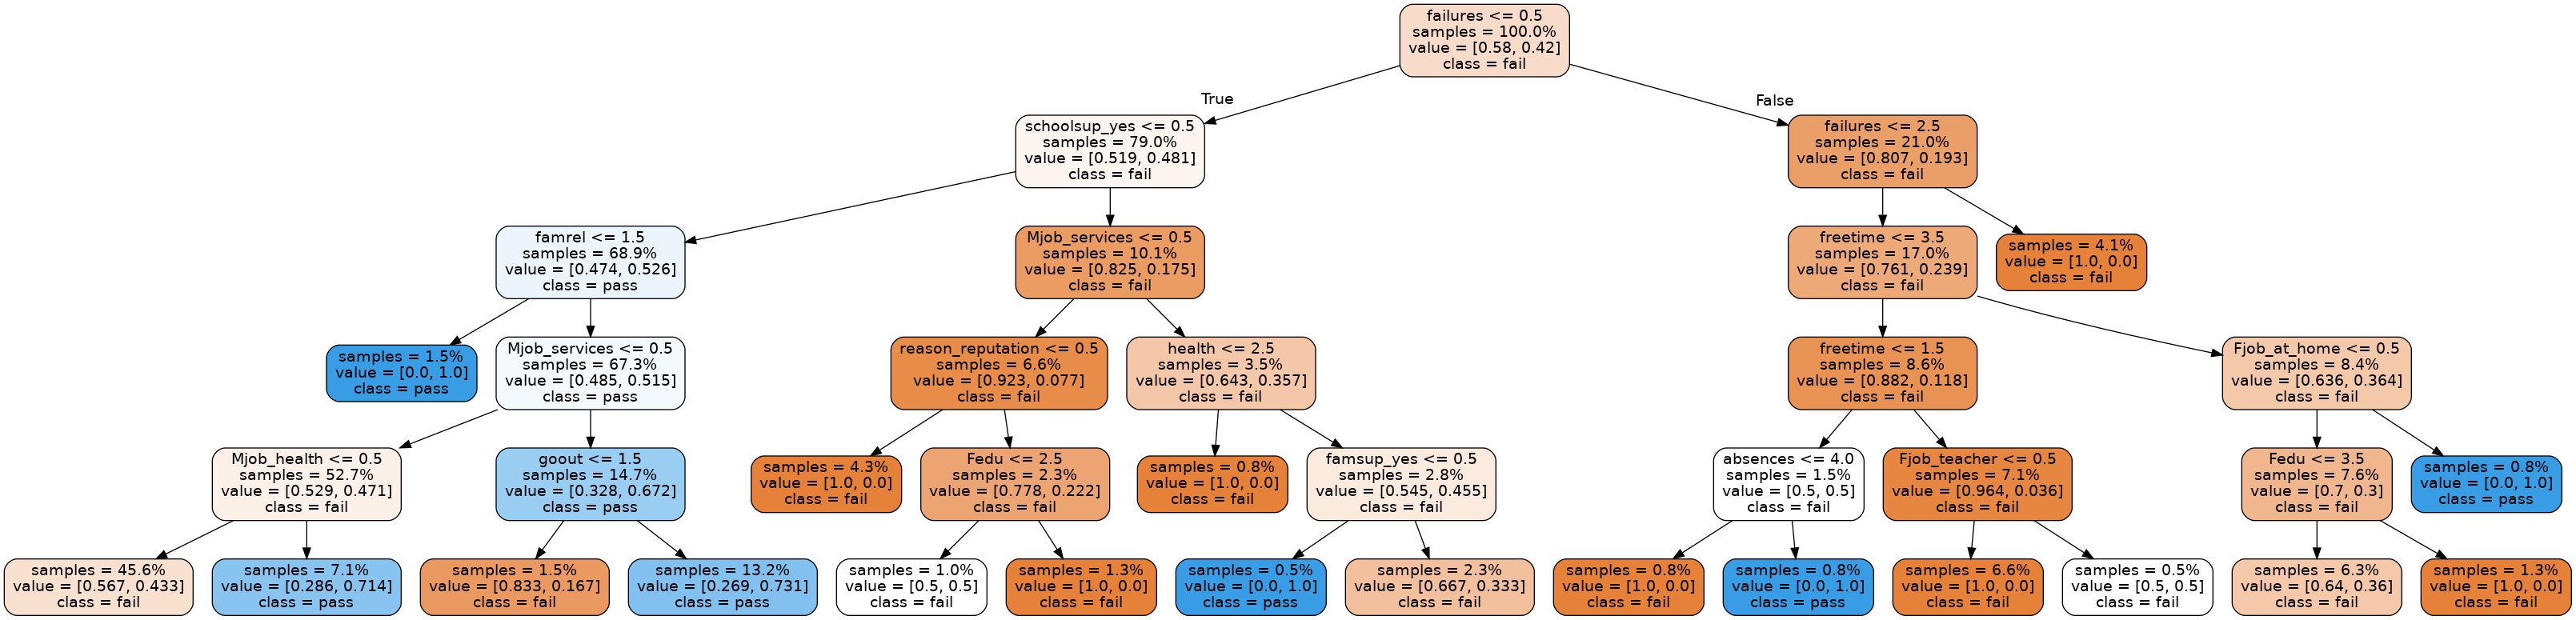
\includegraphics[scale=0.1]{figures/student-performance.PNG}
	\end{figure}
	\item
	Jelaskan apa itu information gain dan entropi dengan gambar ilustrasi buatan sendiri.
	\item 
	\textit{Information Gain} adalah sekumpulan informasi yang didapatkan dari variabel acak.\\
	\textit{Entropi} adalah tingkat keacakan dari informasi yang diperloh dari information gain yang sedang diproses.
\end{itemize}
\end{enumerate}

\section{scikit-learn}
Dataset ambil di https://github.com/PacktPublishing/Python-Artificial-Intelligence-Projects-for-Beginners folder Chapter01.
Tugas anda adalah, dataset ganti menggunakan \textbf{student-mat.csv} dan mengganti semua nama variabel dari kode di bawah ini dengan nama-nama makanan (NPM mod 3=0), kota (NPM mod 3=1), buah (NPM mod 3=2), . Jalankan satu per satu kode tersebut di spyder dengan menggunakan textit{Run current cell}. Kemudian Jelaskan dengan menggunakan bahasa yang mudah dimengerti dan bebas plagiat dan wajib skrinsut dari komputer sendiri masing masing nomor di bawah ini(nilai 5 masing masing pada hari kedua).

\begin{enumerate}

\item
\begin{verbatim}
	#1 Load dataset
	import pandas as pd
	apel = pd.read_csv('student-mat.csv', sep=';')
	len(apel)
\end{verbatim}
	Output :
\begin{figure}[!htbp]
	\centering
	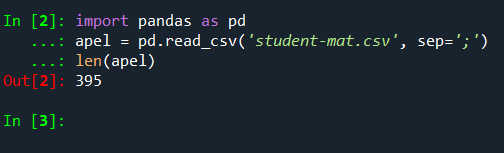
\includegraphics[scale=0.8]{figures/loaddataset1.PNG}
\end{figure}
\item
\begin{verbatim}
	#2 generate binary label (pass)
	# (test grades, each 0-20 pts); threshold for passing is sum>=30
	
	apel['pass'] = apel.apply(lambda row: 1 if (row['G1']+row['G2']+row['G3']) >= 35 else 0, axis=1)
	apel = apel.drop(['G1', 'G2', 'G3'], axis=1)
	apel.head()
\end{verbatim}
	Output :
\begin{figure}[!htbp]
	\centering
	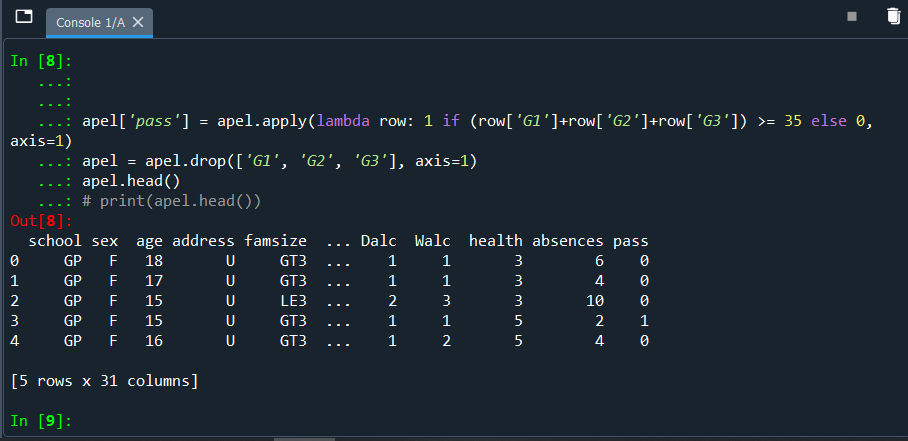
\includegraphics[scale=0.8]{figures/generate_binarylabel.PNG}
\end{figure}
\newpage
\item
\begin{verbatim}
	# 3 use one-hot encoding on categorical columns
	apel = pd.get_dummies(apel, columns=['sex', 'school', 'address', 'famsize', 'Pstatus', 'Mjob', 'Fjob', 
	'reason', 'guardian', 'schoolsup', 'famsup', 'paid', 'activities',
	'nursery', 'higher', 'internet', 'romantic'])
	apel.head()
\end{verbatim}
	Output :
\begin{figure}[!htbp]
	\centering
	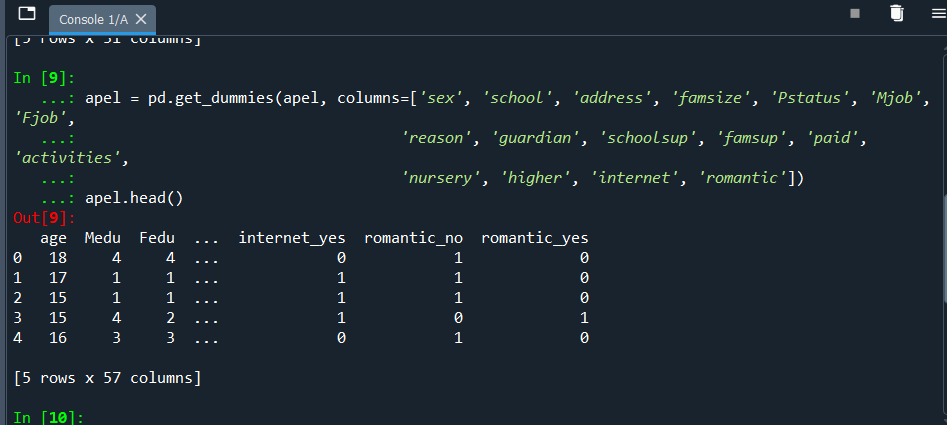
\includegraphics[scale=0.8]{figures/encodingoncategoricalcolumns.PNG}
\end{figure}
\item
\begin{verbatim}
# 4 shuffle rows
apel = apel.sample(frac=1)
#   split traning and testing data
apel_train = apel[:500]
apel_test = apel[:500]

apel_train_att = apel_train.drop(['pass'], axis=1)
apel_train_pass = apel_train['pass']

apel_test_att = apel_test.drop(['pass'], axis=1)
apel_test_pass = apel_test['pass']

apel_att = apel.drop(['pass'], axis=1)
apel_pass = apel['pass']

# number off passing students in whole dataset:
import numpy as np
print("Passing: %d out of %d (%.2f%%)" % (np.sum(apel_pass), len(apel_pass), 
100*float(np.sum(apel_pass)) / len(apel_pass)))
\end{verbatim}
	Output :
\begin{figure}[!htbp]
	\centering
	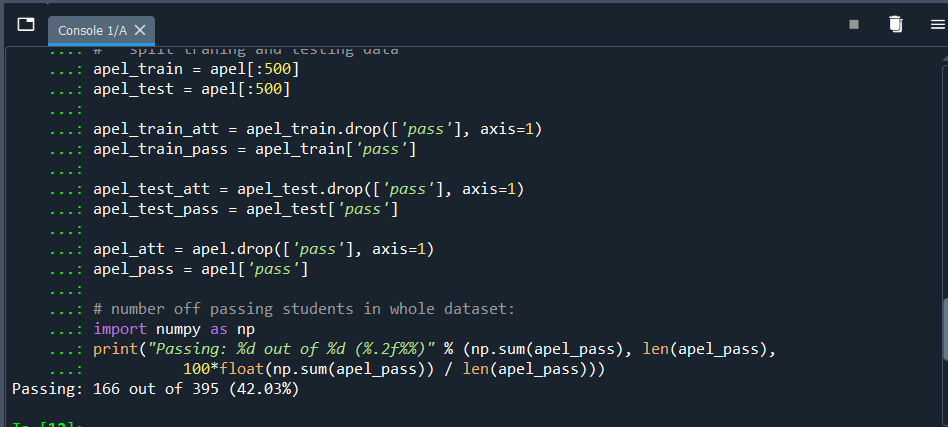
\includegraphics[scale=0.8]{figures/shufflerows.PNG}
\end{figure}
\item 
\begin{verbatim}
	# 5 fit a decision tree
	from sklearn import tree
	semangka = tree.DecisionTreeClassifier(criterion="entropy", max_depth=5)
	semangka = semangka.fit(apel_train_att, apel_train_pass)
\end{verbatim}
\begin{figure}[!htbp]
	\centering
	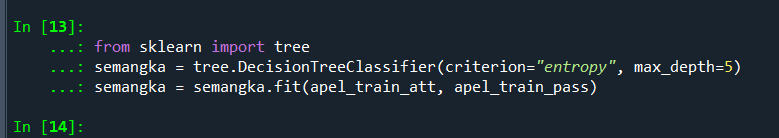
\includegraphics[scale=0.8]{figures/fitdecisontree.PNG}
\end{figure}
\item
\begin{verbatim}
	# 6 visualize tree
	import graphviz
	dot_data = tree.export_graphviz(semangka, out_file=None, label="all", 
	impurity=False, proportion=True,
	feature_names=list(apel_train_att), 
	class_names=["fail", "pass"], 
	filled=True, rounded=True)
	graph = graphviz.Source(dot_data)
	graph
\end{verbatim}
\begin{figure}[!htbp]
	\centering
	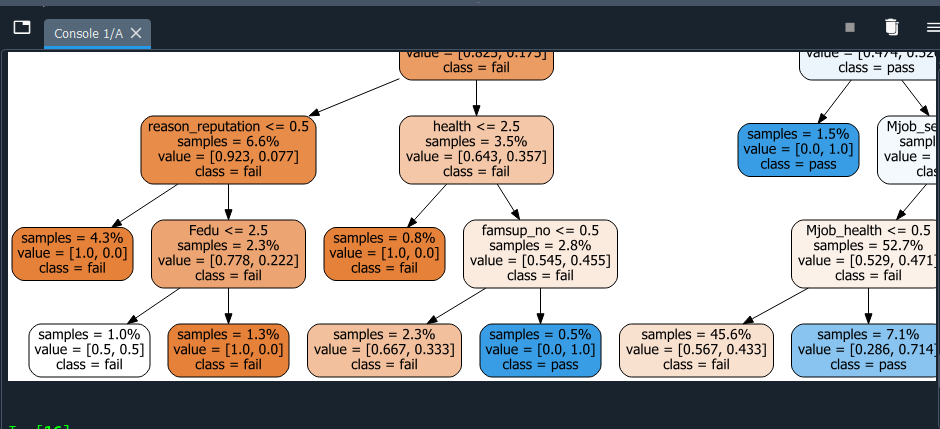
\includegraphics[scale=0.8]{figures/visualizetree.PNG}
\end{figure}
\item
\begin{verbatim}
	# 7 save tree
	tree.export_graphviz(semangka, out_file="student-performance.dot", 
	label="all", impurity=False, 
	proportion=True,
	feature_names=list(apel_train_att), 
	class_names=["fail", "pass"], 
	filled=True, rounded=True)
\end{verbatim}
\begin{figure}[!htbp]
	\centering
	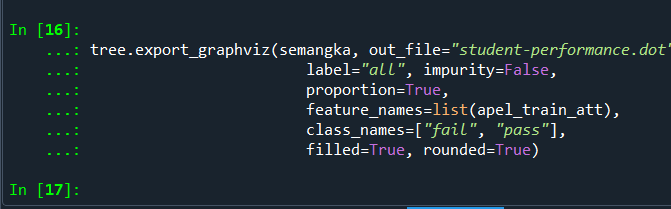
\includegraphics[scale=0.8]{figures/savetree.PNG}
\end{figure}
\item
\begin{verbatim}
	# 8
	semangka.score(apel_test_att, apel_test_pass)
\end{verbatim}
\begin{figure}[!htbp]
	\centering
	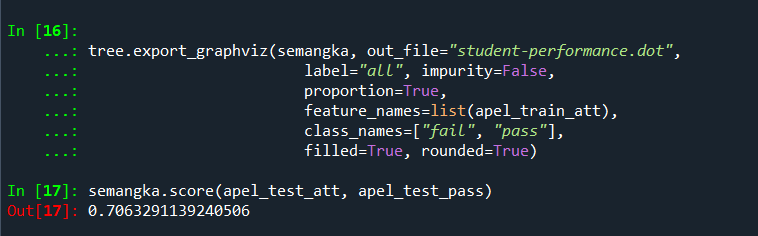
\includegraphics[scale=0.8]{figures/8.PNG}
\end{figure}
\item
\begin{verbatim}
	# 9
	from sklearn.model_selection import cross_val_score
	salak = cross_val_score(semangka, apel_att, apel_pass, cv=5)
	# show average score and +/- two standard deviations away 
	#(covering 95% of scores)
	print("Accuracy: %0.2f (+/- %0.2f)" % (salak.mean(), salak.std() * 2))
\end{verbatim}
\begin{figure}[!htbp]
	\centering
	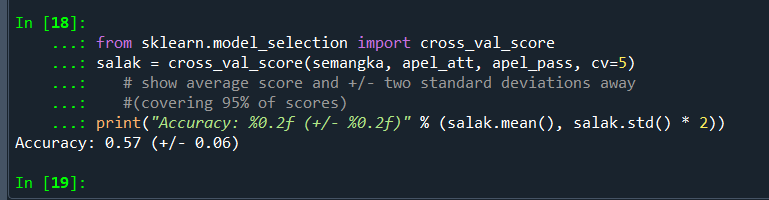
\includegraphics[scale=0.8]{figures/9.PNG}
\end{figure}
\item 
\begin{verbatim}
	# 10
	for max_depth in range(1, 20):
	semangka = tree.DecisionTreeClassifier(criterion="entropy", 
	max_depth=max_depth)
	salak = cross_val_score(semangka, apel_att, apel_pass, cv=5)
	print("Max depth: %d, Accuracy: %0.2f (+/- %0.2f)" % 
	(max_depth, salak.mean(), salak.std() * 2)
	)
\end{verbatim}
\begin{figure}[!htbp]
	\centering
	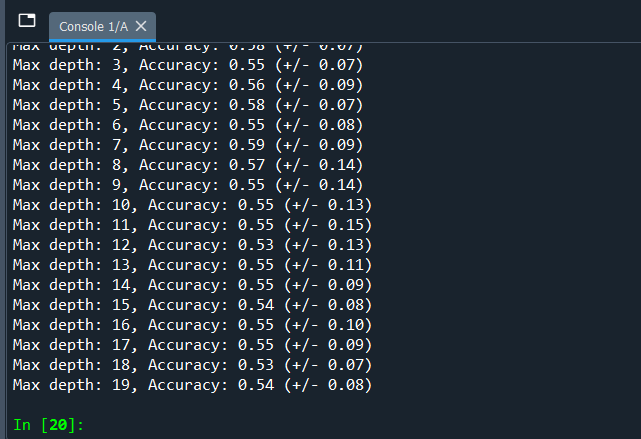
\includegraphics[scale=0.8]{figures/10.PNG}
\end{figure}
\newpage
\item
\begin{verbatim}
	# 11
	depth_acc = np.empty((19,3), float)
	i = 0
	for max_depth in range(1, 20):
	semangka = tree.DecisionTreeClassifier(criterion="entropy", 
	max_depth=max_depth)
	salak = cross_val_score(semangka, apel_att, apel_pass, cv=5)
	depth_acc[i,0] = max_depth
	depth_acc[i,1] = salak.mean()
	depth_acc[i,2] = salak.std() * 2
	i += 1
	depth_acc
\end{verbatim}
\begin{figure}[!htbp]
	\centering
	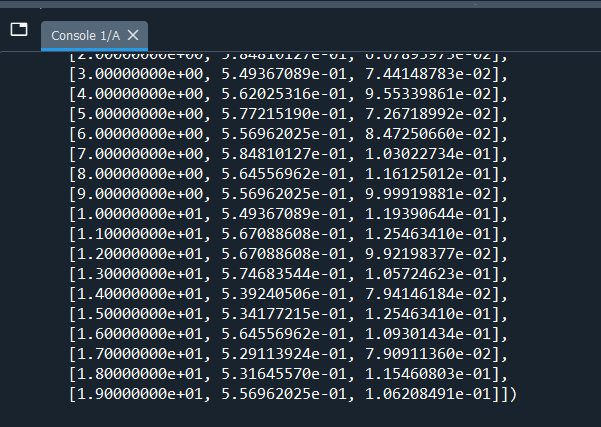
\includegraphics[scale=0.8]{figures/11.PNG}
\end{figure}
\item 
\begin{verbatim}
	# 12
	import matplotlib.pyplot as plt
	fig, ax = plt.subplots()
	ax.errorbar(depth_acc[:,0], depth_acc[:,1], yerr=depth_acc[:,2])
	plt.show()
\end{verbatim}
\begin{figure}[!htbp]
	\centering
	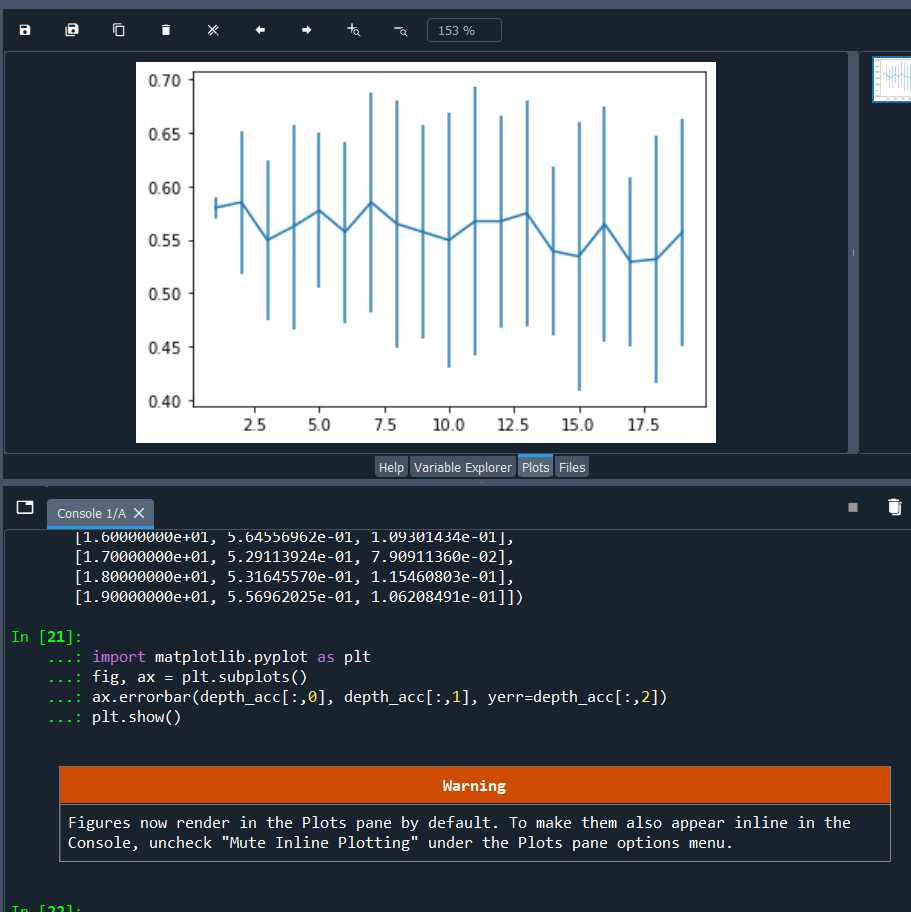
\includegraphics[scale=0.6]{figures/12.PNG}
\end{figure}
\newpage

\end{enumerate}


\section{Penanganan Error}
Dari percobaan yang dilakukan di atas, error yang kita dapatkan di dokumentasikan dan di selesaikan(nilai 5 hari kedua):

\begin{enumerate}
	\item
skrinsut error
\begin{figure}[!htbp]
	\centering
	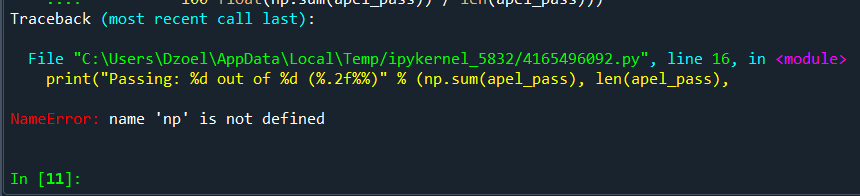
\includegraphics[scale=0.8]{figures/np_not_defined_error.PNG}
\end{figure}
	\item
Tuliskan kode eror dan jenis errornya\\
NameError : name 'np' is not defined
	\item
Solusi pemecahan masalah error tersebut\\
Solusinya adalah import numpy dengan alias np.

\end{enumerate}


%\include{section/chapter3}
%\include{section/chapter4}
%\include{section/chapter5}
%\include{section/chapter6}
%\include{section/chapter7}
%\include{section/chapter8}
%\include{section/chapter9}
%\include{section/chapter10}
%\include{section/chapter11}
%\include{section/chapter12}
%\include{section/chapter13}
%\include{section/chapter14}

%now enable appendix numbering format and include any appendices
%\appendix
%\include{section/appendix1}
%\include{section/appendix2}

%next line adds the Bibliography to the contents page
%\addcontentsline{toc}{chapter}{Bibliography}
%uncomment next line to change bibliography name to references
%\renewcommand{\bibname}{References}
%\bibliography{references}        %use a bibtex bibliography file refs.bib
%\bibliographystyle{plain}  %use the plain bibliography style

\end{document}

